\section{Quantum Phase Estimation}
\subsection{Problem}
Given a unitary operator $U$ and one of its eigen vector $|u\rangle$, determine the phase of the eigen value corresponding to $|u\rangle$. The phase of a unit modulus complex number $e^{2\pi i \phi}$ is $\phi$. Note that the phase $\phi$ will be a fraction between 0 and 1 due to periodicity.\\
\subsection{Solution}
Since the quantum phase estimation is a general problem in the sense that the unitary operator $U$ is not defined, we would assume that we have an oracle which can perform the unitary transformation corresponding to $U$. Further, by using multiple oracles like this, we may form the $Controlled-U^{2^j}$ gate for any non-negative integer $j$. How to make this oracle will depend on the specific application and is not a problem to be considered in the quantum phase estimation.//
Having this oracle and the algorithm to find $QFT^\dagger$ with us, we can solve this problem easily using the following circuit.
\begin{figure}[h]
\centering
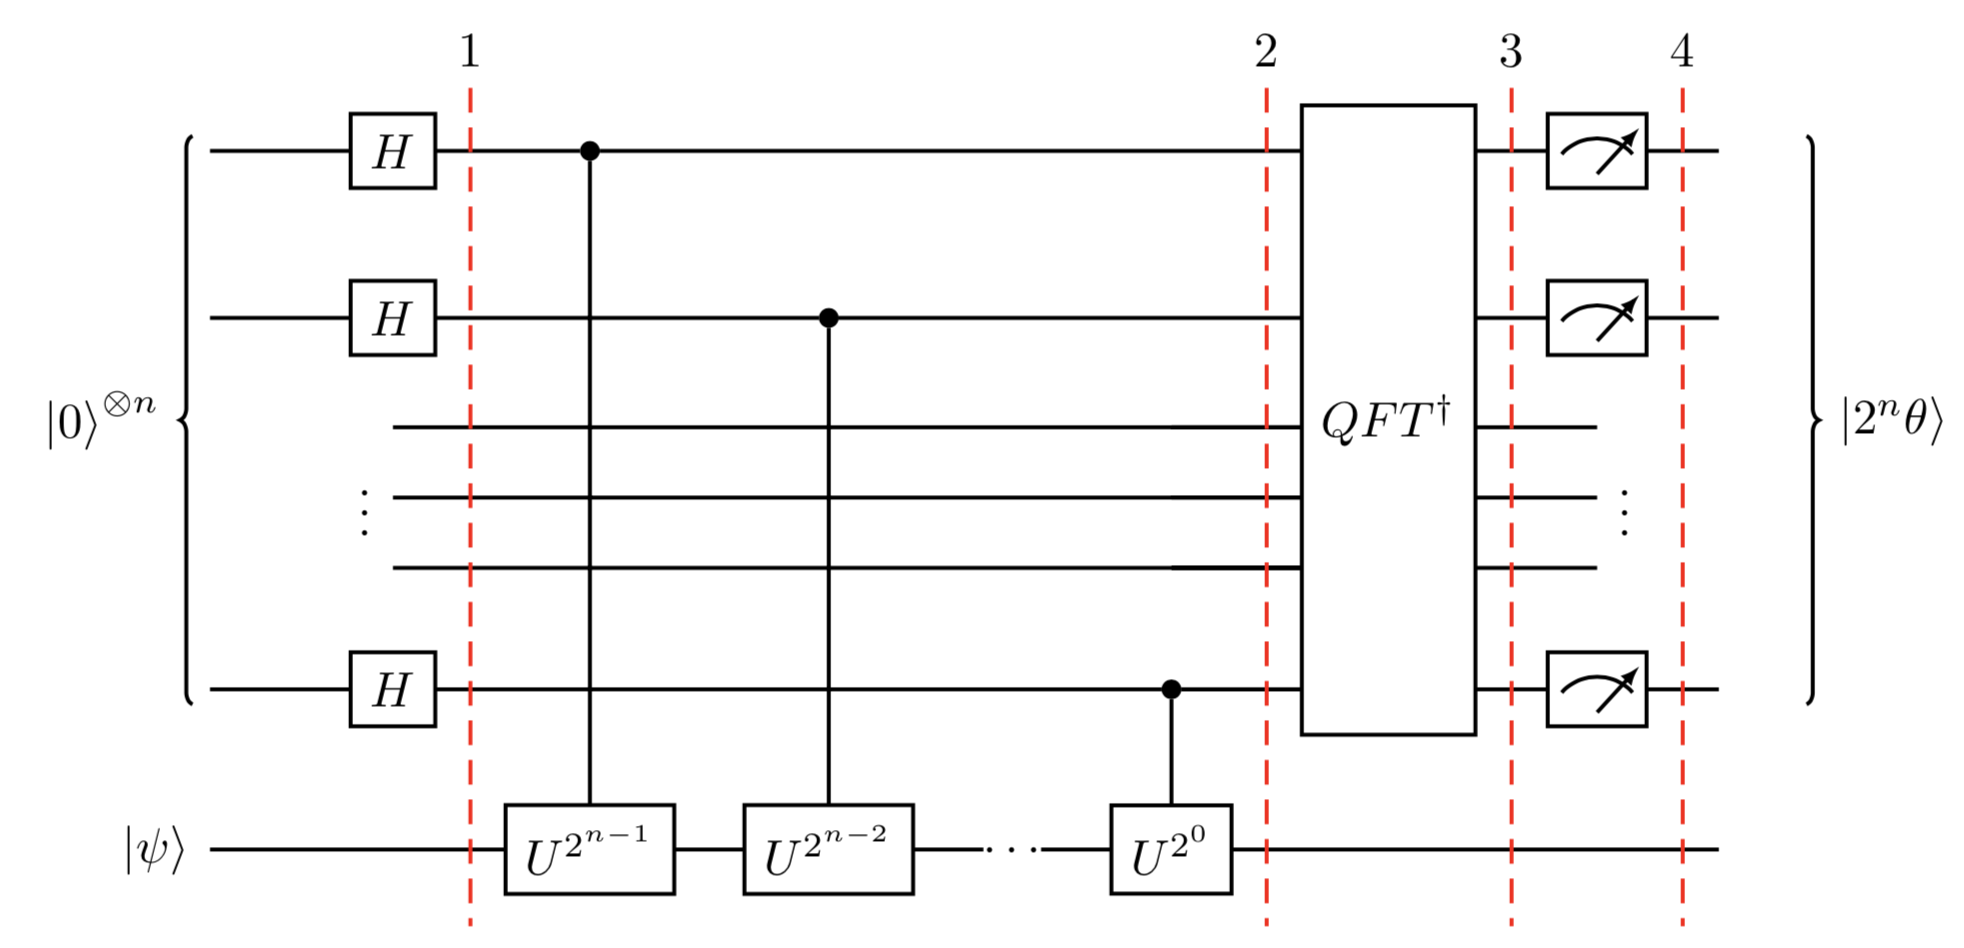
\includegraphics[width=0.9\textwidth]{images/phase.png}
\label{phase}
\caption{Circuit for quantum phase estimation}
\end{figure}
\\We use two registers, one is the output register and the other one contains the eigen vector $|\psi \rangle$. The  size of the output register is determined by how much precision and accuracy is needed in the answer. If we want to estimate the phase to an accuracy of $2^{-x}$ and want the probability of success to be $\epsilon$, then the number of qubits in the output register n, will be
\begin{equation}
n = x + \Bigg\lceil \log{\left( 2 + \frac{1}{2(1-\epsilon)}\right)} \Bigg\rceil
\end{equation}The second term is used to ensure that the result we get is correct with probability 1.
The circuit is divided into 4 parts:
\begin{enumerate}
\item \textbf{Preparing the states:} The initial state taken is $|0\rangle^{\otimes n}|\psi\rangle$ and Hadamard gate is applied on the first register. This is done to get all the possible values of the first register in a superposed state. The transformation is  
\begin{equation}
|0\rangle^{\otimes n} |\psi \rangle \rightarrow \frac{1}{2^{n/2}} \sum_{x=0}^{2^n -1}|x\rangle  |\psi\rangle = \bigotimes_n \left( \frac{|0\rangle + |1\rangle}{\sqrt{2}} \right) |\psi\rangle
\end{equation}
\item \textbf{Applying the operator}: This is the most important part of the phase estimation algorithm. $Controlled-U^{2^{n-j}}$ is applied from the $j^{th}$ qubit of the first register to the second register. Note that the value of the qubits in the first register is $(|0\rangle + |1\rangle)/\sqrt{2}$.  So, the overall operation is:
\begin{equation}
\bigotimes_n \left( \frac{|0\rangle + |1\rangle}{\sqrt{2}} \right) |\psi\rangle \rightarrow \bigotimes_{j=1}^{n} \left( \frac{|0\rangle + e^{2\pi i \phi 2^{n-j}} |1\rangle}{\sqrt{2}} \right) |\psi\rangle 
\end{equation}
Note the value of exponent $2 \pi i \phi 2^{n-j}$. If $0.\phi_1 \phi_2 ... \phi_n$ is the binary representation of the phase $\phi$, then $2^{n-j} \phi$ becomes $\phi_1\phi_2...\phi_{n-j}.\phi_{n-j+1}... \phi_n... $ . But due to the periodic property, it is equivalent to $0.\phi_{n-j+1}... \phi_n..$. So the state becomes:
\begin{equation}
\bigotimes_{j=1}^{n} \left( \frac{|0\rangle + e^{2\pi i 0.\phi_{n-j+1}...\phi_n...} |1\rangle}{\sqrt{2}} \right) |\psi\rangle 
\end{equation}
This is the \textit{product representation} of the Fourier Transform of $|\tilde{\phi}\rangle$. Note that we have denoted it as $\tilde{\phi}$ and not $\phi$. This is because the value may not be represented in $n$ qubits and hence it will be an approximation.
\item \textbf{Inverse Fourier Transform}: This is quite obvious step. So after this step we will get $|\tilde{\phi}\rangle$. Note that the Inverse Fourier transform will not be exact(the binary representation continues after $n$ terms). This leads to some extra terms other than the approximation $|\tilde{\phi}\rangle$ and hence the probability of getting the correct phase approximation may not be 1. Even with this fact, by repeatedly doing the experiment and using some extra qubits(mentioned in the formula for the size of output register), this probability can be made very close to 1.
\item \textbf{Measure}: This step is not necessary if the phase is to be used in some further process. But in case of just quantum phase estimation, we do want to measure the value of the phase. Also, measurement is helpful in removing the extra "noise" terms that occur due to approximate Inverse Fourier Transform.
\end{enumerate}
One drawback of this algorithm is that we must have the eigen vector $|\psi\rangle$. This may be possible in some cases where the eigenvector is obtained as a result of some other operation. But even in case of some other vector, the outcome is not so bad. Let us say that the input $|\psi\rangle = \sum c_j |u_j\rangle$ where $|u_j\rangle$ are the eigen bases. Then this operation will lead to $\sum c_j |\tilde{\phi}_j\rangle |u_j\rangle$ with some noise terms. If we measure the first and the second register both, then there is a high probability that we will get $|\tilde{\phi}_j\rangle |u_j\rangle$ as the output for some $j$. In this way, we would have determined the phase of eigenvalue corresponding to some eigenvector. Repeating this many times, we can get phase for all the eigenbases!!
\newpage
